\documentclass{article}

% Packages
\usepackage[T1]{fontenc}
\usepackage[utf8]{inputenc}
\usepackage[english]{babel}

\usepackage{tikz}
\usepackage{tikzsymbols}
\usetikzlibrary{positioning, math, automata}
\usepackage{amsmath}
\usepackage{graphicx}


\begin{document}

\centering
% M|M|1 example
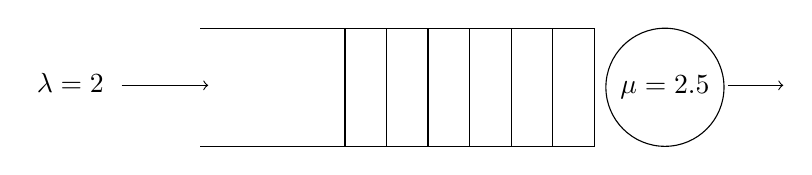
\begin{tikzpicture}
    \draw (2,1.25) -- ++(5cm,0) -- ++(0,-1.5cm) -- ++(-5cm,0);
    \foreach \i in {1,...,6}
    \draw (7cm-\i*15pt,1.25) -- +(0,-1.5cm);
    \draw (7.9,0.5) circle [radius=0.75cm];
    \node[] at (0.7, 0.55) {$\lambda = 2 \qquad$};
    \draw[->] (1, 0.525) -- (2.1, 0.525);
    \node[] at (7.9,0.5) {$\mu = 2.5$};
    \draw[->] (8.7,0.525) -- +(20pt,0);
\end{tikzpicture}

\vspace{2cm}

% M|M|3 example
\begin{tikzpicture} 
    \draw (2,1.25) -- ++(5cm,0) -- ++(0,-1.5cm) -- ++(-5cm,0);
    \foreach \i in {1,...,6}
    \draw (7cm-\i*15pt,1.25) -- +(0,-1.5cm);
    \draw (7.9,-1.1) circle [radius=0.75cm];
    \node[] at (7.9,-1.1) {$\mu = 0.8$};
    \draw (7.9,0.5) circle [radius=0.75cm];
    \node[] at (7.9,0.5) {$\mu = 0.8$};
    \draw (7.9,2.1) circle [radius=0.75cm];
    \node[] at (7.9,2.1) {$\mu = 0.8$};
    \node[] at (0.7, 0.55) {$\lambda = 2 \qquad$};
    \draw[->] (1, 0.525) -- (2.1, 0.525);
    \draw[->] (8.7,0.525) -- +(20pt,0);
\end{tikzpicture}

\vspace{2cm}

% Two waiting spaces example
\begin{tikzpicture}[>=stealth] %arrow type
    % the rectangle with vertical rules (Queue 1)
    \draw (0,0) -- ++(2cm,0) -- ++(0,-1.5cm) -- ++(-2cm,0);
    \foreach \i in {1,...,4}
    \draw (2cm-\i*10pt,0) -- +(0,-1.5cm);
    
    % the circle (Queue 1)
    \draw (2.75,-0.75cm) circle [radius=0.75cm];

    % the rectangle with vertical rules (Queue 2)
    \draw (5,1.25) -- ++(2cm,0) -- ++(0,-1.5cm) -- ++(-2cm,0);
    \foreach \i in {1,...,4}
    \draw (7cm-\i*10pt,1.25) -- +(0,-1.5cm);
    
    % The two vertical lines at the very start of Queue 2 
    \draw (7cm-54pt,1.2) -- +(0,-0.5cm);
    \draw (7cm-54pt,0.3) -- +(0,-0.5cm);        
    \draw (7cm-51pt,1.1) -- +(0,-0.4cm);
    \draw (7cm-51pt,0.3) -- +(0,-0.4cm);
    
    % The label between the lines for T
    \node[anchor=north] at (5.15, 0.75 cm) {\small{\( 10 \)}};
    
    % the circle (Queue 2)
    \draw (7.9, 2.1) circle [radius=0.75cm];
    \node[] at (7.9, 2.1) {$\mu = 2$};
    \draw (7.9, 0.5) circle [radius=0.75cm];
    \node[] at (7.9, 0.5) {$\mu = 2$};
    \draw (7.9, -1.1) circle [radius=0.75cm];
    \node[] at (7.9, -1.1) {$\mu = 2$};

    % the arrows and labels (Queue 1+2)
    \draw[->] (8.7,0.525) -- +(20pt,0);
    \node[align=center] at (1cm,-2cm) {};
    \node[align=center] at (6cm,-0.75cm) {};
    
    % Ambulance lines
    \draw[<-] (0,-0.75) -- +(-50pt,0) node[left] {\( \lambda_2 = 2 \)};
    \draw[-] (3.5,-0.75) -- +(20pt,0);
    \draw (4.2, 0.525) -- (4.2, -0.75);

    % Others lines
    \draw (4.2, 1.8) -- +(-169.5pt,0) node[left] {\( \lambda_1 = 3\)};
    \draw (4.2, 1.8) -- (4.2, 0.525);
    \draw[->] (4.2, 0.525) -- (5, 0.525);

\end{tikzpicture}


    
\end{document}